% DO NOT COMPILE THIS FILE DIRECTLY!
% This is included by the other .tex files.

\begin{frame}[t,plain]
\titlepage
\end{frame}

\begin{frame}
\frametitle{Indicators - Problem Statement}
    \begin{itemize}
            \item Various users and organisations can share data via MISP, multiple parties can be involved
        \begin{itemize}
            \item Trust, data quality and time-to-live issues
            \item Each user/organisation has different use-cases and interests
        \end{itemize}
        \vspace{0.5cm}
        \item Attributes can be shared in large quantities (more than 1.3 million on \texttt{MISPPRIV})
        \begin{itemize}
            \item Partial info about their validity (sightings)
            \item Partial info about their freshness (last update)
            \item Varius conflicting interests such as operational security, attribution, source reliability evaluation...
        \end{itemize}
    \end{itemize}
\end{frame}

\begin{frame}
\frametitle{Sightings - Refresher}
    Sightings add temporal context to indicators.
    A user, script or an IDS can extend the information related to indicators by reporting back to MISP that
    an indicator has been \texttt{seen}, or that an indicator can be considered as a \texttt{false-positive}
    \vspace{0.5cm}
    \begin{itemize}
        \item Sightings give more credibility/visibility to indicators
        \item This information can be used to {\bf prioritise and decay indicators}
    \end{itemize}
\end{frame}

\begin{frame}
\frametitle{Organisations opt-in - setting a level of confidence}
    MISP is a peer-to-peer system, information passes through multiple instances.
    \begin{itemize}
            \item Producers can add context (such as tags from taxonomies, galaxies) about their asserted confidence or the reliability of the data
        \item Consumers can have different levels of trust in the producers and/or analysts themselves
    \end{itemize}

    \begin{small}
    \begin{columns}[T] % align columns
    \begin{column}{.40\textwidth}
        \begin{tabular}{|ll|}
            \hline
            \textbf{Description} & \textbf{Value}\\
            \hline
            Completely reliable & 100\\
            Usually reliable & 75\\
            Fairly reliable & 50\\
            Not usually reliable & 25\\
            Unreliable & 0\\
            Reliability cannot be judged & 50\\
            Deliberatly deceptive & 0\\
            \hline
        \end{tabular}
    \end{column}%
    \hfill%
    \begin{column}{.48\textwidth}
        \begin{tabular}{|ll|}
            \hline
            \textbf{Description} & \textbf{Value}\\
            \hline
            Confirmed by other sources & 100\\
            Probably true & 75\\
            Possibly true & 50\\
            Doubtful & 25\\
            Improbable & 0\\
            Truth cannot be judged & 50\\
            \hline
        \end{tabular}
    \end{column}%
    \end{columns}
    \end{small}
\end{frame}

\begin{frame}
        \frametitle{Scoring Indicators 1/2}
        When scoring indicators\footnote{Paper available: \url{https://arxiv.org/pdf/1803.11052}}, multiple parameters\footnote{at a variable extent as required} can be taken into account. The {\bf base score} is calculated with the following in mind:
    \begin{itemize}
        \item The reliability in the producer
        \item The trust in the data as signaled by the producer
        $$base\_score = weigth_{tg} \cdot tags + \omega_{sc} \cdot source\_confidence$$
    \end{itemize}
\end{frame}

\begin{frame}
        \frametitle{Scoring Indicators 2/2}
        The weighted score is calculated using:
        \begin{itemize}
        \item The lifetime of the indicator (e.g. IP address vs hash value of a file)
            \begin{itemize}
                \item The lifespan of the indicator (short for an IP - long for an hash): $\tau$
                \item The decay rate $\rightarrow$ Speed at which an attribute loses value: $\delta$
                \item Weigthed score is reset to its base score as new \texttt{sightings} are received
            \end{itemize}
            $$score = base\_score \cdot \left( 1 - \left( \frac{t}{\tau_a} \right)^{\frac{1}{\delta_a}} \right) $$
        \end{itemize}
\end{frame}

\begin{frame}
\frametitle{Ongoing Implementation in MISP}
    Setting thresholds and retrieving the information should be simple and straightforward for the user:
    \begin{itemize}
        \item Automatic scoring based on default values
        \item User-friendly UI to manually set lifetime parameters
        \item Interaction through the API
    \end{itemize}
    \begin{center}
        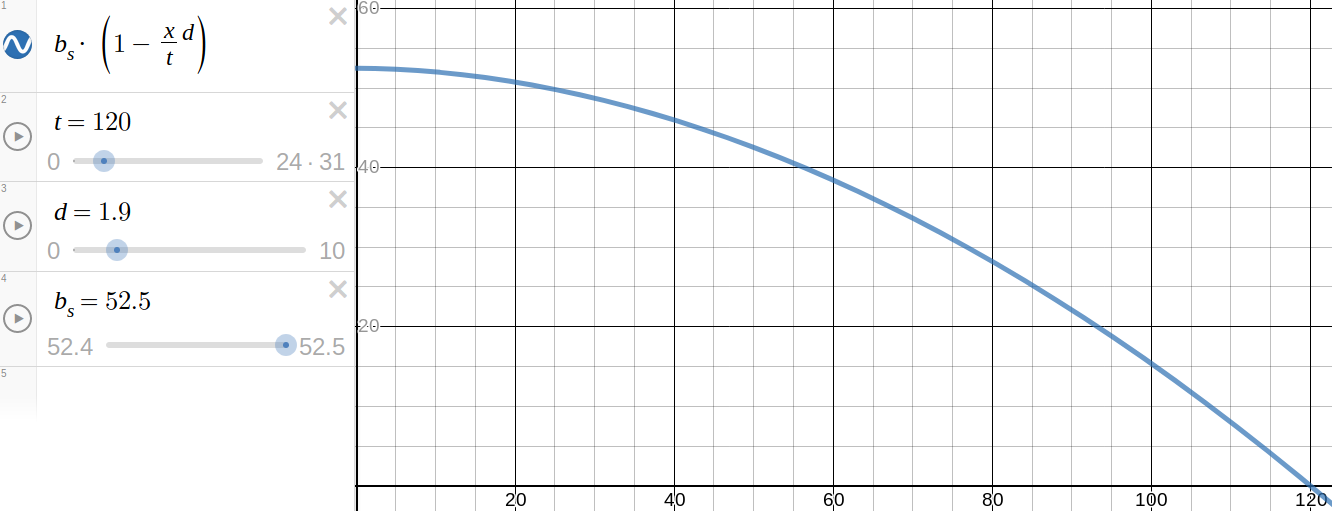
\includegraphics[scale=0.15]{pics/param-ui.png}
    \end{center}
\end{frame}
